
\section{Алгоритмы поиска по аналогии части речи и грамсета}\label{section:pos_algorithm}

Алгоритмы работают по данным морфологического словаря.
В основе алгоритмов лежит гипотеза, что слова с \emph{одинаковыми конечными буквосочетаниями} с высокой вероятностью имеют одинаковые словоизменительные модели и одинаковые наборы грамматической информации (часть речи, число, падеж, время, лицо и др.).
%The \emph{suffix} here is a final segment of a string of characters.

Исходя из такой гипотезы, грамматическую информацию для «новых» (несловарных) слов можно определять по аналогии со словами, уже включенными в машинный словарь, при условии, что конечные буквосочетания новых слов совпадают с конечными буквосочетаниями слов из словаря.

Пусть гипотеза верна, тогда если суффиксы новых слов совпадают с суффиксами словарных слов, тогда часть речи и грамматические свойства новых слов будут совпадать со словарными словами.
При этом длина совпадающих буквосочетаний не регламентируется и для разных пар слов может быть различной~\cite[p.~53]{Belonogov2004}.

Описанные далее алгоритмы POSGuess и GramGuess используют понятие <<конечное буквосочетание>> 
(рис.~\ref{fig:kezaman_substring}), 
алгоритм GramPseudoGuess --- <<псевдоокончание>> (рис.~\ref{fig:huukkua_substring}).


\subsection{Алгоритм POSGuess поиска части речи по конечным буквосочетаниям}

Дано множество словоформ $W$,  в котором для каждой словоформы известна часть речи. Алгоритм~\ref{alg:POSGuess} ищет часть речи $\pos_u$ для заданного слова~$u$, используя это множество.

%\newpage
\begin{algorithm}%[H]
    \caption{Алгоритм поиска части речи по конечным буквосочетаниям (POSGuess)}
    \label{alg:POSGuess}
\DontPrintSemicolon
\SetAlgoLined
    \KwData{
        $P$ -- a set of part of speech (POS),\hfill \break
        $W = \{ w \; | \; \exists \pos_w \in P \}$ -- a set of words, POS is known for each word,\hfill \break
        %$S = \{ s \; | \; s=\{w, p_w\}, w \in W, p_w \in P \}$ -- a set of 
        %    relations \{word, POS\},\hfill \break
        $u \notin W$ -- the word with unknown POS,\hfill \break
        $len(u)$ -- the length (in characters) of the string $u$.
       }
    \KwResult{\[
        u_z : 
        \begin{cases}
            %z = \underset{z \in [2, len(u)], 
            %              z \in \mathbb{Z}^+}{\mathrm{argmax}} \; len(u_z)\\
            %
            len (u_z) \xrightarrow[ z=2,\ldots,len(u) ]{} \max,\;
            % \textcolor{blue}{u_z} - 
            \Comment{//\,Longest suffix}\\
            \exists w \in W : w = w_{\text{prefix}} \concat u_z\;
            \Comment{//\,Concatenation of strings}
        \end{cases}
        \]
    \begin{align*}
\text{Counter} & \left[ \pos^k \right] = c^k, \; k = \overline{1,m}, \; \text{where :}\\
        & c^k \in \mathbb{N}, \; c^1 \geq c^2 \geq \ldots \geq c^m,\\
        & \exists w^k_i \in W : 
            w^k_i = {w_{\text{prefix}}}^k_i \concat u_z \Rightarrow
            c^k = \vert \pos^k_{w^k_i} \vert, \\
        &    
            i = \overline{1,c^k}, \\
        & \forall i : \pos^k_{w^k_i} = \pos^k \in P, \;\;\;\; 
           a \ne b \Leftrightarrow \pos^a \ne \pos^b\\
        & 
        m \; \text{-- the number of different POS of found words} \; w^k_i
    \end{align*}
  %\hfill \break
    } % eo KwResult
    %\BlankLine
    
    $z$ = 2 \Comment{// The position in the string $u$}
    $z_{found} = \text{FALSE}$ \;
    \BlankLine
    \While{ $z \leq len(u)$ and $\neg z_{found}$ }{
        \BlankLine
        \Comment{// The suffix of the word $u$ from $z$-th character}
        $u_z = \text{ substr } (u, z) \;$
        \BlankLine
        \ForEach{$w \in W$}{
            \Comment{// If the word $w$ has the suffix $u_z$ (regular expression)
            }
            \If{$w =\sim \textrm{m}/u_z\$/$}{
                $\text{Counter} \left[ \pos_w \right] ++$\\
                $z_{found} = \text{TRUE}$ \Comment{// Only POS of words with this $u_z$ suffix will be counted. The next ``while'' loop will break, so the shorter suffix $u_{z+1}$ will be omitted.}
% Only parts of the speech of those words that have this suffix $u_z$ will be counted. 
            }
        }
    z = z + 1
    }
    \BlankLine
    \Comment{// Sort the array in descending order, according to the value}
    \verb|arsort|( $\text{Counter} \left[ \; \right]$ )
\end{algorithm}

%\newpage

% Последовательно перебираем подстроки u, начиная от самой длинной (подстрока со второго до последнего символа) до подстроки из одного символа.
В алгоритме~\ref{alg:POSGuess} мы ищем в множестве $W$ (строка~5) слова, имеющие такие же конечные буквосочетания $u_z$ как и  у несловарного слова $u$. 
Сначала мы ищем самую длинную подстроку у $u$, начинающуюся с индекса $z$. 
Первая подстрока $u_{z=2}$ начинается со второго символа (строка 1 в алгоритме~\ref{alg:POSGuess}), в то время как $u_{z=1} = u$~--- это вся строка (рис.~\ref{fig:kezaman_substring}). 

Потом мы в цикле увеличиваем на единицу значение $z$, уменьшая длину подстроки $u_z$, 
пока подстрока $u_z$ имеет ненулевую длину, $z \leq len(u)$.
Если находятся слова из множества $W$ с таким же конечным буквосочетанием, то мы считаем количество подобных слов для каждой части речи и останавливаем поиск.

\begin{figure}
    \centering
	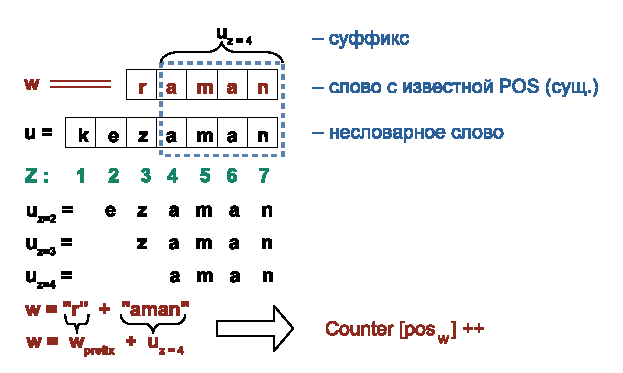
\includegraphics[width=0.7\textwidth,keepaspectratio=true]{kezaman_substring}
	\caption[Сравнение конечных буквосочетаний в алгоритме POSGuess]{Сравнение 
конечных буквосочетаний в алгоритме POSGuess на примере 
вепсских существительных в генетиве ``kezaman'' (талая земля) и ``raman'' (оправа). 
	Слово $u$ 
	с неизвестной частью речи~--- ``kezaman''. 
	Слово $w$ из словаря с известной частью речи (POS)~--- ``raman''. 
	Они имеют одинаковое конечное буквосочетание $u_z$~--- ``aman''.} 
	\label{fig:kezaman_substring}
\end{figure}

%\hfill \break

На рис. 2 показана идея работы алгоритма~\ref{alg:POSGuess}: в алгоритме для нового слова ($kezaman$) мы ищем слово в словаре ($raman$), с таким же конечным буквосочетанием ($aman$). 

При этом мы ищем в словаре такое слово, чтобы совпал самое длинное конечное буквосочетание несловарного слова. То есть начинаем искать в словаре слова, оканчивающиеся на $u_{z=2}$ . Если не находим, то ищем $u_{z=3}$ и так далее.
В примере было найдено слово при  $z=4$ с конечным буквосочетанием $u_{z=4}$=``aman''.

Теперь мы переберем все слова из $W$, оканчивающиеся на $u_{z=4}$ и подсчитаем, сколько из таких слов существительных, глаголов, наречий и т.д.. 
Результат подсчёта запишем в массив $Counter[\,]$. На рис.~\ref{fig:kezaman_substring} найдено \emph{существительное} ``raman'', поэтому увеличиваем на единицу счётчик $Counter[noun]$.

Сортируем массив по значениям в убывающем порядке (строка~13). Та часть речи, которая встретится чаще с таким конечным буквосочетанием будет на первом месте в массиве $Counter[noun]$, это и есть наиболее вероятная часть речи для слова $u$.


\subsection{Алгоритм GramGuess поиска грамсета по конечным буквосочетаниям}

Алгоритм GramGuess подобен алгоритму POSGuess за исключением того, что для несловарного слова вместо части речи нужно определить набор грамматических признаков.
То есть в множестве $W$ для каждого слова известна морфологическая информация (грамсет\footnote{См. полный список грамсетов на сайте корпуса ВепКар \url{http://dictorpus.krc.karelia.ru/en/dict/gramset}}): число, падеж, время и т.д.


\subsection{Алгоритм GramPseudoGuess поиска грамсета по псевдоокончаниям}

Объясним понятие <<псевдоокончание>>, используемое в алгоритме GramPseudoGuess.
Алгоритм GramPseudoGuess построен на идее, что у словоформ, принадлежащих одной лемме 
есть одинаковая неизменяемая часть~--- \emph{псевдооснова} и это всегда начало строки. 
Например, на рис.~\ref{fig:huukkua_substring} псевдооснова~--- это неизменяемая часть ``huuk'' 
для всех словоформ леммы ``huukkua'' (карельский глагол <<аукать>>).
%Here the pseudo-base is placed at the start of a word, it suits for the Veps and Karelian languages.

Тогда \emph{псевдоокончание} словоформы - это та часть строки, которая останется, если от начала <<отрезать>> псевдооснову.  
Таким образом, любую словоформу можно рассматривать как конкатенацию строк: превдооснова + псевдоокончание. 
Причем псевдооснова~--- одинаковая последовательность символов для всех словоформ одной парадигмы.

\begin{figure}
    \centering
    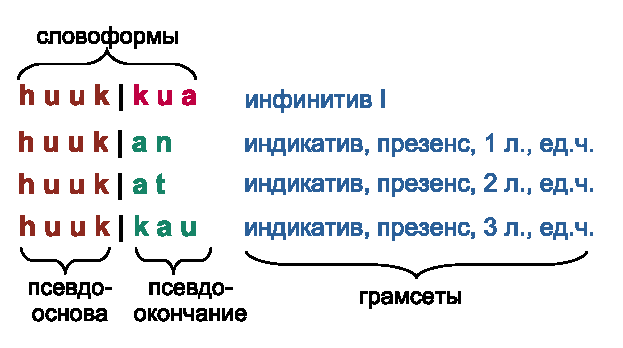
\includegraphics[width=0.5\textwidth]{huukkua_substring}
    \caption[Словоформы карельского глагола ``huukkua'']{Словоформы карельского глагола ``huukkua'' (окликать, аукать). 
    Все словоформы имеют одинаковую псевдооснову и различные псевдоокончания 
    для различных наборов грамматических признаков (грамсетов).} 
    \label{fig:huukkua_substring}
% TODO нарисовать картинку для третьего алгоритма, 
% где для неизвестного слова u
% поочерёдно подбираются существующие слова из словаря 
% со всё укарачивающимся псевдоокончанием...
\end{figure}

Дано множество слов $W$,  в котором для каждого слова известны грамсет и псевдоокончание. Алгоритм~\ref{alg:POSPseudoGuess} ищет грамсет $g_u$ для заданного слова~$u$, используя это множество.

%\newpage
\begin{algorithm}%[H]
    \caption{Gramset search by a pseudo-ending (GramPseudoGuess)}
    \label{alg:POSPseudoGuess}
\DontPrintSemicolon
\SetAlgoLined
    \KwData{
        $G$ -- a set of gramsets,\hfill \break
        $W = \{ w \; | \; \exists \,g_w \in G, 
                \exists \,\pend_w : w = w_{\text{prefix}} \concat \pend_w \}$ 
                -- a set of words, where gramset and pseudo-ending (pend) are known for each word,  \hfill \break
        %$S = \{ s \; | \; s=\{w, p_w\}, w \in W, p_w \in P \}$ -- a set of 
        %    relations \{word, POS\},\hfill \break
        $u \notin W$ -- the word with unknown gramset,\hfill \break
        $len(u)$ -- the length (in characters) of the string $u$.
       }
    \KwResult{\[
        u_z : 
        \begin{cases}
            %z = \underset{z \in [2, len(u)], 
            %              z \in \mathbb{Z}^+}{\mathrm{argmax}} \; len(u_z)\\
            %
            len (u_z) \xrightarrow[ z=2,\ldots,len(u) ]{} \max,\;
            % \textcolor{blue}{u_z} - 
            \Comment{//\,Longest substring}\\
            \exists w \in W : \pend_w = u_z\;
        \end{cases}
        \]
    \begin{align*}
\text{Counter} & \left[ g^k \right] = c^k, \; k = \overline{1,m}, \; \text{where :}\\
        & c^k \in \mathbb{N}, \; c^1 \geq c^2 \geq \ldots \geq c^m,\\
        & \exists w^k_i \in W : 
            \pend_{w^k_i} = u_z \Rightarrow
            c^k = \vert g^k_{w^k_i} \vert, \\
        &    
            i = \overline{1,c^k}, \\
        & \forall i : g^k_{w^k_i} = g^k \in G, \;\;\;\; 
           a \ne b \Leftrightarrow g^a \ne g^b\\
        & 
        m \; \text{-- the number of different gramsets of found words} \; w^k_i
    \end{align*}
    %\hfill \break
    } % eo KwResult
    \BlankLine
    
    $z$ = 2 \Comment{// The position in the string $u$}
    $z_{found} = \text{FALSE}$ \;
    \BlankLine
    \While{ $z \leq len(u)$ and $\neg z_{found}$ }{
        \BlankLine
        \Comment{// The substring of the word $u$ from $z$-th character}
        $u_z = \text{ substr } (u, z) \;$
        \BlankLine
        \ForEach{$w \in W$}{
            \Comment{// If the word $w$ has the pseudo-ending $u_z$}
            \If{$\pend_w == u_z$}{
                $\text{Counter} \left[ g_w \right] ++$\\
                $z_{found} = \text{TRUE}$ \Comment{// Only gramsets of words with the pseudo-ending $u_z$ will be counted. The next "while" loop will break, so the shorter $u_{z+1}$ will be omitted.}
            }
        }
    z = z + 1
    }
    \BlankLine
    \Comment{// Sort the array in descending order, according to the value}
    \verb|arsort|( $\text{Counter} \left[ \; \right]$ )
\end{algorithm}

% Последовательно перебираем подстроки u, начиная от самой длинной (подстрока со второго до последнего символа) до подстроки из одного символа.
В алгоритме~\ref{alg:POSPseudoGuess} 
мы ищем в множестве $W$ (line~5) слова, имеющие псевдоокончания, совпадающие с псевдоокончанием $u_z$ несловарного слова $u$. 
Сначала мы ищем самую длинную подстроку у $u$, начинающуюся с индекса z. 

Потом мы в цикле увеличиваем значение $z$, уменьшая длину подстроки $u_z$, пока 
подстрока $u_z$ имеет ненулевую длину, $z \leq len(u)$.
Если в множестве $W$ находятся слова с таким же псевдоокончанием, то мы считаем количество подобных слов для каждого грамсета и останавливаем поиск.